\def\rescaledTetraTikz{
\begin{figure}[!ht]
  \centering
    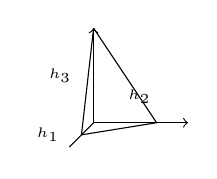
\begin{tikzpicture}[scale=.4]
      \draw[->] (0, 0, 0) -- node[label={above:$_{_{h_2}}$}] { } (3,0,0);
      \draw[->] (0, 0, 0) -- node[label={left:$_{_{h_3}}$}] { } (0, 3, 0);
      \draw (0, 0, 1) -- (2, 0, 0); 
%      \draw (0, 3.5, 1) -- (2, 3.5, 0); 
      \draw (2, 0, 0) -- (0, 3, 0);
      \draw (0, 0, 1) -- (0, 3, 0); 
      \draw (0,0,2) -- node[label={left:$_{_{h_1}}$}] { }  (0,0,0) ;
      %\draw (0,3.5,0) -- (2,3.5,0);
    \end{tikzpicture}
  \caption{Rescaled Tetrahedron}
  \label{rescaled_tetra}    
\end{figure}
}

\newcommand{\referenceTriangleTikz}[1]{
\begin{tikzpicture}[scale={#1}]
  \draw (0,0,0) -- (1.2,0,0);
	\draw (0,0,0) -- (0,1.2,0); 
  \draw (1,0,0) -- (0,1,0);
  \draw[white] (1.2,0,0) -- (1.5,0,0);
  \draw[white] (0,0,0) -- (0,0,.7);
\end{tikzpicture}
}

\newcommand{\referencePrismTikz}[1]{
\begin{tikzpicture}[scale={#1}]
  \draw (0, 0, 0) -- (0, 0, 1); 
  \draw (0, 0, 0) -- (1, 0, 0);
  \draw (0, 0, 0) -- (0, 1, 0);
	\draw (0, 0, 1) -- (1, 0, 0);
	\draw (0, 1, 1) -- (1, 1, 0);
	\draw (1, 0, 0) -- (1, 1, 0);
	\draw (0, 0, 1) -- (0, 1, 1);
	\draw (0, 1, 1) -- (0,1,0);
	\draw (0, 1, 0) -- (1,1,0);
\end{tikzpicture}
}

\newcommand{\referencePyramidTikz}[1]{
\begin{tikzpicture}[scale={#1}]
  \coordinate (o) at (0,0,0);
  \coordinate (e1) at (0,0,1);
  \coordinate (e2) at (1,0,0);
  \coordinate (e3) at (0,1,0);

  \draw (o) -- (e1) -- ($(e1)+(e2)$) -- (e2) -- (e3) -- 
      (o)-- (e2);
  \draw (e3) -- (e1);
  \draw (e3) -- ($(e1)+(e2)$);
  \draw[white] (e1) -- ($1.4*(e1)$);
  \draw[white] (e2) -- ($1.2*(e2)$);
\end{tikzpicture}
}

\newcommand{\referenceTetrahedronTikz}[1]{
\begin{tikzpicture}[scale={#1}]
  \coordinate (o) at (0,0,0);
  \coordinate (e1) at (0,0,1);
  \coordinate (e2) at (1,0,0);
  \coordinate (e3) at (0,1,0);

  \draw (o) -- (e1) -- (e2) -- (o) -- (e3) -- (e2);
  \draw (e3) -- (e1);

\end{tikzpicture}
}

\def\macroRegularity{  
\begin{figure}
  \centering
  \subfloat[Prismatic Macroelement.]
  {
    \label{macro_prism_reg}
    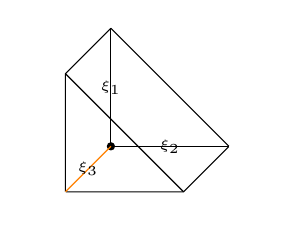
\begin{tikzpicture}[scale=1.5]
      \draw[white] (0,0,0) -- (-.7,0,0);
      \draw[white] (1,0,0) -- (1.4,0,0);
      \fill[black] (0,0,0) circle (1pt);
      \draw (0,0,0) -- node[midway] {\tiny{\color{black}$\xi_1$}} (0,1,0);
      \draw (0,0,0) -- node[midway] {\tiny{\color{black}$\xi_2$}} (1,0,0);
      \draw (0,1,0) -- (1,0,0) -- (1,0,1) -- (0,0,1);
      \draw (0,1,0) -- (0,1,1) -- (0,0,1);
      \draw (1,0,1) -- (0,1,1);
      \draw[orange] (0,0,0) -- node[midway] {\tiny{\color{black}$\xi_3$}} (0,0,1);
      \draw[white] (0,0,1) -- (0,0,1.5);
      \draw[white] (1,0,0) -- (1.3,0,0);
    \end{tikzpicture}
  }
  \hspace{1.5cm}
  \subfloat[Tetrahedral Macro\-ele\-ment.]
  {
    \label{macro_tetra_reg}
    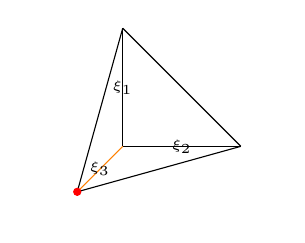
\begin{tikzpicture}[scale=1.5]
      \draw[white] (-.8,0,0) -- (1.3,0,0);
      \draw (0,0,0) -- node[midway] {\tiny{\color{black}$\xi_1$}} (0,1,0);
      \draw (0,0,0) -- node[midway] {\tiny{\color{black}$\xi_2$}} (1,0,0);
      \draw (0,1,0) -- (1,0,0);
      \draw[orange] (0,0,0) -- node[midway] {\tiny{\color{black}$\xi_3$}} (0,0,1);
      \draw[white] (0,0,1) -- (0,0,1.5);
      \draw (0,1,0) -- (0,0,1);
      \draw (1,0,0) -- (0,0,1);
      \fill[red] (0,0,1) circle (1pt);
    \end{tikzpicture}
  }  
  \caption{Macroelements.}
\end{figure}
}

\def\unitTangentsPyramid{
\begin{tikzpicture}[scale=2,post/.style={->, shorten >=1pt, >=stealth', semithick}]
  \coordinate (o) at (0,0,0);
  \coordinate (e1) at (0,0,1);
  \coordinate (e2) at (1,0,0);
  \coordinate (e3) at (0,1,0);
  \coordinate (e4) at ($(e1)+(e2)$);

  \coordinate (a1start) at ($.2*(e1)$);
  \coordinate (a1end)   at ($.5*(e1)$);
  \coordinate (a2start)   at ($.8*(e1)+.2*(e4)$);
  \coordinate (a2end)   at ($.5*(e1)+.5*(e4)$);
  \coordinate (a3start)   at ($.8*(e2)+.2*(e4)$);
  \coordinate (a3end)   at ($.5*(e2)+.5*(e4)$);
  \coordinate (a4start) at ($.17*(e2)$);
  \coordinate (a4end)   at ($.4*(e2)$);
  \coordinate (a5start) at ($.2*(e3)$);
  \coordinate (a5end)   at ($.5*(e3)$);
  \coordinate (a6start) at ($.2*(e3)+.8*(e1)$);
  \coordinate (a6end)   at ($.5*(e3)+.5*(e1)$);
  \coordinate (a7start) at ($.2*(e3)+.8*(e2)$);
  \coordinate (a7end)   at ($.5*(e3)+.5*(e2)$);
  \coordinate (a8start) at ($.2*(e3)+.8*(e4)$);
  \coordinate (a8end)   at ($.5*(e3)+.5*(e4)$);

  \draw (o) -- (e1) -- ($(e1)+(e2)$) -- (e2) -- (e3) -- 
      (o)-- (e2);
  \draw (e3) -- (e1);
  \draw (e3) -- (e4);
  \foreach \i in {1,...,8}{
    \draw [post,very thick] (a\i start) -- (a\i end);
  }

\end{tikzpicture}
}

\def\unitTangentsPrism{
\begin{tikzpicture}[scale=2,post/.style={->, shorten >=1pt, >=stealth', semithick}]
  \coordinate (o) at (0,0,0);
  \coordinate (e1) at (0,0,1);
  \coordinate (e2) at (1,0,0);
  \coordinate (e3) at (0,1,0);
  \coordinate (e4) at ($(e1)+(e3)$);
  \coordinate (e5) at ($(e2)+(e3)$);

  \coordinate (a1start) at ($.2*(e1)$);
  \coordinate (a1end)   at ($.5*(e1)$);
  \coordinate (a2start)   at ($.2*(e2)$);
  \coordinate (a2end)   at ($.5*(e2)$);

  \coordinate (a3start)   at ($.2*(e3)$);
  \coordinate (a3end)   at ($.5*(e3)$);

  \coordinate (a4start) at ($.83*(e3)+.17*(e4)$);
  \coordinate (a4end)   at ($.5*(e3)+.5*(e4)$);
  
  \coordinate (a5start) at ($.8*(e3)+.2*(e5)$);
  \coordinate (a5end)   at ($.5*(e3)+.5*(e5)$);
  
  \coordinate (a6start) at ($.2*(e4)+.8*(e1)$);
  \coordinate (a6end)   at ($.5*(e4)+.5*(e1)$);
  \coordinate (a7start) at ($.2*(e5)+.8*(e2)$);
  \coordinate (a7end)   at ($.5*(e5)+.5*(e2)$);
  \coordinate (a8start) at ($.2*(e4)+.8*(e5)$);
  \coordinate (a8end)   at ($.5*(e4)+.5*(e5)$);
  \coordinate (a9start) at ($.2*(e1)+.8*(e2)$);
  \coordinate (a9end)   at ($.5*(e1)+.5*(e2)$);

  \draw (o) -- (e1) -- (e2) -- (o) -- (e3) -- (e4) -- (e5) -- (e3);
  \draw (e4) -- (e1);
  \draw (e5) -- (e2);

  \foreach \i in {1,...,9}{
    \draw [post, very thick] (a\i start) -- (a\i end);
  }
\end{tikzpicture}
}

\newcommand{\prismaticMacroelement}[5]{
\def\m{#1} % piso y tapa como m-'agonos
\def\n{#2} % (n + 1) puntos en cada arista del tri'angulo
\def\mu{#3} % graduaci'on
\def\init{#4} % hacia d'onde queremos que apunte la boca

\foreach \l in {0,...,\n} {
  \pgfmathparse{-\l*2/\n} \let\L\pgfmathresult
  %\pgfmathparse{\m + \init - 2} \let\last\pgfmathresult
  %%% TODO perspectiva: hacer unos defs con los canonicos y el entero 1, 2, 3 de entrada
  %\pgfmathparse{\n + 1} \let\N\pgfmathresult
  \begin{scope}[shift={(0,\L,0)}]   %% --->>> altura
    \coordinate (point1) at ({cos((.15+\init-2)*\twoPi/\m)},0,{sin((.15+\init-2)*\twoPi/\m)});  %% -->> perspectiva
    \coordinate (point2) at ({cos((.15+\init-1)*\twoPi/\m)},0,{sin((.15+\init-1)*\twoPi/\m)});
    \draw[color=#5] (point1) -- (point2);

    \pgfmathparse{\n-1} \let\to\pgfmathresult
    \foreach \i in {0,...,\to} {  
      \pgfmathparse{pow(\i/\n,1/\mu)} \let\rad\pgfmathresult
      \draw[color=#5] ($\rad*(point1)$) -- ($\rad*(point2)$);
      
      \pgfmathparse{\n-\i-1} \let\ni\pgfmathresult
      \foreach \j in {0,...,\ni} {
        \pgfmathparse{(\i/\n)*pow((\i+\j)/\n,1/\mu-1)} \let\alfa\pgfmathresult
        \pgfmathparse{(\j/\n)*pow((\i+\j)/\n,1/\mu-1)} \let\beta\pgfmathresult

        \pgfmathparse{(\i/\n)*pow((\i+(\j+1))/\n,1/\mu-1)}    \let\alfaSuc\pgfmathresult
        \pgfmathparse{((\j+1)/\n)*pow((\i+(\j+1))/\n,1/\mu-1)}  \let\betaSuc\pgfmathresult
        
        \draw[color=#5] ($\alfa*(point1) + \beta*(point2)$) -- 
            ($\alfaSuc*(point1) + \betaSuc*(point2)$);
        \draw[color=#5] ($\alfa*(point2) + \beta*(point1)$) -- 
            ($\alfaSuc*(point2) + \betaSuc*(point1)$);
      };
    }
  \end{scope}
  }
  \coordinate (point1) at ({cos((.15+\init-2)*\twoPi/\m)},0,{sin((.15+\init-2)*\twoPi/\m)});
  \coordinate (point2) at ({cos((.15+\init-1)*\twoPi/\m)},0,{sin((.15+\init-1)*\twoPi/\m)}); 
  \pgfmathparse{\n} \let\to\pgfmathresult
  \foreach \i in {0,...,\to} {  
    \pgfmathparse{\n-\i} \let\ni\pgfmathresult
    \foreach \j in {0,...,\ni} {
      \pgfmathparse{(\i/\n)*pow((\i+\j)/\n,1/\mu-1)} \let\alfa\pgfmathresult
      \pgfmathparse{(\j/\n)*pow((\i+\j)/\n,1/\mu-1)} \let\beta\pgfmathresult
      \pgfmathparse{(\i/\n)*pow((\i+(\j+1))/\n,1/\mu-1)}    \let\alfaSuc\pgfmathresult
      \pgfmathparse{((\j+1)/\n)*pow((\i+(\j+1))/\n,1/\mu-1)}  \let\betaSuc\pgfmathresult        
      \draw[color=#5] ($\alfa*(point1) + \beta*(point2)$) -- 
        ($\alfa*(point1)+ \beta*(point2) + (0,-2,0)$); 
   };
  };
  \draw[red] (0,0,0) -- (0,-2,0);
}

\def\prismsBaryCoordA{
\begin{table}
  \centering  
  \caption{{Barycentric coordinates of prismatic mesh points} in $\Lambda_\ell$
   \newline $0\leqslant l\leqslant n-2$, $i+j\leqslant n-l-2$}
  \label{prisms_barycentric_a}
  \begin{IEEEeqnarraybox*}
    [\IEEEeqnarraystrutmode
    \IEEEeqnarraystrutsizeadd{2pt}{6pt}]{v/c/v/c/v/c/v/c/v/c/v/}
      \IEEEeqnarrayrulerow\\
      \IEEEeqnarrayseprow[5pt]\\
         & p_0 && {\scriptstyle 1-\left(\frac{n-l}n\right)^{\nicefrac{1}{\mu}}      } 
               && {\scriptstyle \left(\frac{n-l}n\right)^{\nicefrac{1}{\mu}}-\left(\frac{i+j}n\right)^{\nicefrac{1}{\mu}}   }
               && {\scriptstyle \frac in \left(\frac{i+j}n\right)^{\nicefrac{1}{\mu}-1}   }
               && {\scriptstyle \frac jn \left(\frac{i+j}n\right)^{\nicefrac{1}{\mu}-1} }
         & \\
      \IEEEeqnarrayrulerow\\
      \IEEEeqnarrayseprow[5pt]\\
         & p_1 && {\scriptstyle 1-\left(\frac{n-l}n\right)^{\nicefrac{1}{\mu}}} 
               && {\scriptstyle \left(\frac{n-l}n\right)^{\nicefrac{1}{\mu}}-\left(\frac{i+j+1}n\right)^{\nicefrac{1}{\mu}} }
               && {\scriptstyle \frac{i+1}n \left(\frac{i+1+j}n\right)^{\nicefrac{1}{\mu}-1} }
               && {\scriptstyle \frac jn \left(\frac{i+1+j}n\right)^{\nicefrac{1}{\mu}-1} }
         & \\
      \IEEEeqnarrayrulerow\\
      \IEEEeqnarrayseprow[5pt]\\
         & p_2 && {\scriptstyle 1-\left(\frac{n-l}n\right)^{\nicefrac{1}{\mu}} }
               && {\scriptstyle \left(\frac{n-l}n\right)^{\nicefrac{1}{\mu}}-\left(\frac{i+j+1}n\right)^{\nicefrac{1}{\mu}} }
               && {\scriptstyle \frac in \left(\frac{i+j+1}n\right)^{\nicefrac{1}{\mu}-1} }
               && {\scriptstyle \frac{j+1}n \left(\frac{i+1+j}n\right)^{\nicefrac{1}{\mu}-1}}
         & \\
      \IEEEeqnarrayrulerow\\
      \IEEEeqnarrayseprow[5pt]\\
         & p_3 && {\scriptstyle 1-\left(\frac{n-l-1}n\right)^{\nicefrac{1}{\mu}} }
               && {\scriptstyle \left(\frac{n-l-1}n\right)^{\nicefrac{1}{\mu}}-\left(\frac{i+j}n\right)^{\nicefrac{1}{\mu}} }
               && {\scriptstyle \frac in \left(\frac{i+j}n\right)^{\nicefrac{1}{\mu}-1} }
               && {\scriptstyle \frac jn \left(\frac{i+j}n\right)^{\nicefrac{1}{\mu}-1}}
         & \\
      \IEEEeqnarrayrulerow\\
      \IEEEeqnarrayseprow[5pt]\\
         & p_4 && {\scriptstyle 1-\left(\frac{n-l-1}n\right)^{\nicefrac{1}{\mu}} }
               && {\scriptstyle \left(\frac{n-l-1}n\right)^{\nicefrac{1}{\mu}}-\left(\frac{i+1+j}n\right)^{\nicefrac{1}{\mu}} }
               && {\scriptstyle \frac{i+1}n \left(\frac{i+1+j}n\right)^{\nicefrac{1}{\mu}-1} }
               && {\scriptstyle \frac jn \left(\frac{i+1+j}n\right)^{\nicefrac{1}{\mu}-1}}
         & \\
      \IEEEeqnarrayrulerow\\
      \IEEEeqnarrayseprow[5pt]\\
         & p_5 && {\scriptstyle 1-\left(\frac{n-l-1}n\right)^{\nicefrac{1}{\mu}} }
               && {\scriptstyle \left(\frac{n-l-1}n\right)^{\nicefrac{1}{\mu}}-\left(\frac{i+j+1}n\right)^{\nicefrac{1}{\mu}} }
               && {\scriptstyle \frac in \left(\frac{i+j+1}n\right)^{\nicefrac{1}{\mu}-1} }
               && {\scriptstyle \frac{j+1}n \left(\frac{i+1+j}n\right)^{\nicefrac{1}{\mu}-1}}
         & \\
      \IEEEeqnarrayrulerow
  \end{IEEEeqnarraybox*}
\end{table}}

\def\prismsBaryCoordB{
\begin{table}
  \centering  
  \caption{{Barycentric coordinates of prismatic mesh points} in $\Lambda_\ell$
  \newline $0\leqslant l\leqslant n-2,\qquad i\ge1, \qquad \mbox{and}\qquad i+j\leqslant n-l-2$}
  \label{prisms_barycentric_b}
  \begin{IEEEeqnarraybox*}
    [\IEEEeqnarraystrutmode
    \IEEEeqnarraystrutsizeadd{2pt}{6pt}]{v/c/v/c/v/c/v/c/v/c/v/}
      \IEEEeqnarrayrulerow\\
      \IEEEeqnarrayseprow[5pt]\\
         & p_0  && {\scriptstyle 1-\left(\frac{n-l}n\right)^{\nicefrac{1}{\mu}}      } 
               && {\scriptstyle \left(\frac{n-l}n\right)^{\nicefrac{1}{\mu}}-\left(\frac{i+j}n\right)^{\nicefrac{1}{\mu}}   }
               && {\scriptstyle \frac in \left(\frac{i+j}n\right)^{\nicefrac{1}{\mu}-1}   }
               && {\scriptstyle \frac jn \left(\frac{i+j}n\right)^{\nicefrac{1}{\mu}-1} }
         & \\
      \IEEEeqnarrayrulerow\\
      \IEEEeqnarrayseprow[5pt]\\
         & p_1  && {\scriptstyle 1-\left(\frac{n-l}n\right)^{\nicefrac{1}{\mu}} }  
               && {\scriptstyle \left(\frac{n-l}n\right)^{\nicefrac{1}{\mu}}-\left(\frac{i+j+1}n\right)^{\nicefrac{1}{\mu}} }
               && {\scriptstyle \frac in \left(\frac{i+j+1}n\right)^{\nicefrac{1}{\mu}-1} }
               && {\scriptstyle   \frac{j+1}n \left(\frac{i+j+1}n\right)^{\nicefrac{1}{\mu}-1}}
         & \\
      \IEEEeqnarrayrulerow\\
      \IEEEeqnarrayseprow[5pt]\\
         & p_2 && {\scriptstyle 1-\left(\frac{n-l}n\right)^{\nicefrac{1}{\mu}}  }
               && {\scriptstyle \left(\frac{n-l}n\right)^{\nicefrac{1}{\mu}}-\left(\frac{i+j}n\right)^{\nicefrac{1}{\mu}} }
               && {\scriptstyle \frac{i-1}n \left(\frac{i+j}n\right)^{\nicefrac{1}{\mu}-1} }
               && {\scriptstyle \frac{j+1}n \left(\frac{i+j}n\right)^{\nicefrac{1}{\mu}-1}}
         & \\
      \IEEEeqnarrayrulerow\\
      \IEEEeqnarrayseprow[5pt]\\
         & p_3  && {\scriptstyle 1-\left(\frac{n-l-1}n\right)^{\nicefrac{1}{\mu}} }
               && {\scriptstyle \left(\frac{n-l-1}n\right)^{\nicefrac{1}{\mu}}-\left(\frac{i+j}n\right)^{\nicefrac{1}{\mu}} }
               && {\scriptstyle \frac in \left(\frac{i+j}n\right)^{\nicefrac{1}{\mu}-1} }
               && {\scriptstyle   \frac jn \left(\frac{i+j}n\right)^{\nicefrac{1}{\mu}-1}}
         & \\
      \IEEEeqnarrayrulerow\\
      \IEEEeqnarrayseprow[5pt]\\
         & p_4 && {\scriptstyle 1-\left(\frac{n-l-1}n\right)^{\nicefrac{1}{\mu}} }
               && {\scriptstyle \left(\frac{n-l-1}n\right)^{\nicefrac{1}{\mu}}-\left(\frac{i+j+1}n\right)^{\nicefrac{1}{\mu}} }
               && {\scriptstyle \frac in \left(\frac{i+j+1}n\right)^{\nicefrac{1}{\mu}-1} }
               && {\scriptstyle \frac{j+1}n \left(\frac{i+j+1}n\right)^{\nicefrac{1}{\mu}-1}}
         & \\
      \IEEEeqnarrayrulerow\\
      \IEEEeqnarrayseprow[5pt]\\
         & p_5  && {\scriptstyle 1-\left(\frac{n-l-1}n\right)^{\nicefrac{1}{\mu}} }
               && {\scriptstyle \left(\frac{n-l-1}n\right)^{\nicefrac{1}{\mu}}-\left(\frac{i+j}n\right)^{\nicefrac{1}{\mu}} }
               && {\scriptstyle \frac{i-1}n \left(\frac{i+j}n\right)^{\nicefrac{1}{\mu}-1} }
               && {\scriptstyle \frac{j+1}n \left(\frac{i+j}n\right)^{\nicefrac{1}{\mu}-1}}
         & \\
      \IEEEeqnarrayrulerow
  \end{IEEEeqnarraybox*}
\end{table}}

\def\pyramidsBaryCoord{
\begin{table}
  \centering  
  \caption{Barycentric coordinates of pyramidal mesh points in $\Lambda_\ell$.
      \newline
    $0\leqslant l\leqslant n-2 \qquad\mbox{and}\qquad 1\leqslant i\leqslant n-l-1.$
      \newline}
  \label{pyramidal_barycentric}
  \begin{IEEEeqnarraybox*}
    [\IEEEeqnarraystrutmode
    \IEEEeqnarraystrutsizeadd{2pt}{6pt}]{v/c/v/c/v/c/v/c/v/c/v/}
      \IEEEeqnarrayrulerow\\
      \IEEEeqnarrayseprow[5pt]\\
         & p_0 && {\scriptstyle 1-\left(\frac{n-l}n\right)^{\nicefrac{1}{\mu}}  }
               && {\scriptstyle \left(\frac{n-l}n\right)^{\nicefrac{1}{\mu}}-\left(\frac{n-l-1}n\right)^{\nicefrac{1}{\mu}}  }
               && {\scriptstyle \frac in \left(\frac{n-l-1}n\right)^{\nicefrac{1}{\mu}-1}  }
               && {\scriptstyle \frac{n-l-i-1}n \left(\frac{n-l-1}n\right)^{\nicefrac{1}{\mu}-1}}
         & \\
      \IEEEeqnarrayrulerow\\
      \IEEEeqnarrayseprow[5pt]\\
         & p_1 && {\scriptstyle 1-\left(\frac{n-l}n\right)^{\nicefrac{1}{\mu}} }
               && {\scriptstyle \left(\frac{n-l}n\right)^{\nicefrac{1}{\mu}}-\left(\frac{n-l-1}n\right)^{\nicefrac{1}{\mu}} }
               && {\scriptstyle \frac{i-1}n \left(\frac{n-l-1}n\right)^{\nicefrac{1}{\mu}-1} }
               && {\scriptstyle \frac{n-l-i}n \left(\frac{n-l-1}n\right)^{\nicefrac{1}{\mu}-1}}
         & \\
      \IEEEeqnarrayrulerow\\
      \IEEEeqnarrayseprow[5pt]\\
         & p_2 && {\scriptstyle 1-\left(\frac{n-l-1}n\right)^{\nicefrac{1}{\mu}}  }
               && {\scriptstyle   0  }
               && {\scriptstyle   \frac in \left(\frac{n-l-1}n\right)^{\nicefrac{1}{\mu}-1}  }
               && {\scriptstyle   \frac{n-l-i-1}n \left(\frac{n-l-1}n\right)^{\nicefrac{1}{\mu}-1}}
         & \\
      \IEEEeqnarrayrulerow\\
      \IEEEeqnarrayseprow[5pt]\\
         & p_3 && {\scriptstyle 1-\left(\frac{n-l-1}n\right)^{\nicefrac{1}{\mu}}  }
               && {\scriptstyle 0  }
               && {\scriptstyle \frac{i-1}n \left(\frac{n-l-1}n\right)^{\nicefrac{1}{\mu}-1}  }
               && {\scriptstyle \frac{n-l-i}n \left(\frac{n-l-1}n\right)^{\nicefrac{1}{\mu}-1}}
         & \\
      \IEEEeqnarrayrulerow\\
      \IEEEeqnarrayseprow[5pt]\\
         & p_4 && {\scriptstyle 1-\left(\frac{n-l}n\right)^{\nicefrac{1}{\mu}}  }
               && {\scriptstyle 0  }
               && {\scriptstyle \frac in \left(\frac{n-l}n\right)^{\nicefrac{1}{\mu}-1}  }
               && {\scriptstyle \frac{n-l-i}n \left(\frac{n-l}n\right)^{\nicefrac{1}{\mu}-1}}
         & \\
      \IEEEeqnarrayrulerow
  \end{IEEEeqnarraybox*}
\end{table}}

\def\tetrahedraBaryCoord{
\begin{table}
  \centering  
  \caption{Barycentric coordinates of tetrahedral mesh points in $\Lambda_\ell$.
      \newline
$0\leqslant l\leqslant n-1\qquad\mbox{and}\qquad 1\leqslant i\leqslant n-l-1$
      \newline}
  \label{tetrahedral_barycentric}
  \begin{IEEEeqnarraybox*}
    [\IEEEeqnarraystrutmode
    \IEEEeqnarraystrutsizeadd{2pt}{6pt}]{v/c/v/c/v/c/v/c/v/c/v/}
      \IEEEeqnarrayrulerow\\
      \IEEEeqnarrayseprow[5pt]\\
         & p_0 && {\scriptstyle 1-\left(\frac{n-l}n\right)^{\nicefrac{1}{\mu}} }
               && {\scriptstyle \left(\frac{n-l}n\right)^{\nicefrac{1}{\mu}}-\left(\frac{n-l-1}n\right)^{\nicefrac{1}{\mu}} }
               && {\scriptstyle \frac in \left(\frac{n-l-1}n\right)^{\nicefrac{1}{\mu}-1} }
               && {\scriptstyle \frac{n-l-i-1}n \left(\frac{n-l-1}n\right)^{\nicefrac{1}{\mu}-1}}
         & \\
      \IEEEeqnarrayrulerow\\
      \IEEEeqnarrayseprow[5pt]\\
         & p_1 && {\scriptstyle 1-\left(\frac{n-l-1}n\right)^{\nicefrac{1}{\mu}}  }
               && {\scriptstyle 0  }
               && {\scriptstyle \frac in \left(\frac{n-l-1}n\right)^{\nicefrac{1}{\mu}-1}  }
               && {\scriptstyle \frac{n-l-i-1}n \left(\frac{n-l-1}n\right)^{\nicefrac{1}{\mu}-1}}
         & \\
      \IEEEeqnarrayrulerow\\
      \IEEEeqnarrayseprow[5pt]\\
         & p_2 && {\scriptstyle 1-\left(\frac{n-l}n\right)^{\nicefrac{1}{\mu}}  }
               && {\scriptstyle 0  }
               && {\scriptstyle \frac in \left(\frac{n-l}n\right)^{\nicefrac{1}{\mu}-1}  }
               && {\scriptstyle \frac{n-l-i}n \left(\frac{n-l}n\right)^{\nicefrac{1}{\mu}-1}}
         & \\
      \IEEEeqnarrayrulerow\\
      \IEEEeqnarrayseprow[5pt]\\
         & p_3 && {\scriptstyle 1-\left(\frac{n-l}n\right)^{\nicefrac{1}{\mu}}  }
               && {\scriptstyle 0  }
               && {\scriptstyle \frac{i+1}n \left(\frac{n-l}n\right)^{\nicefrac{1}{\mu}-1}  }
               && {\scriptstyle \frac{n-l-i-1}n \left(\frac{n-l}n\right)^{\nicefrac{1}{\mu}-1}}
         & \\
      \IEEEeqnarrayrulerow
  \end{IEEEeqnarraybox*}
\end{table}}

%\def\prismsProductCoord{
%\begin{table}
%  \centering  
%  \caption{Cartesian coordinates of prismatic mesh points in $\Lambda_\ell$.
%      \newline
%$0\leqslant l\leqslant n-1\qquad\mbox{and}\qquad 1\leqslant i\leqslant n-l-1$
%      \newline}
%  \label{prisms_product}
%  \begin{IEEEeqnarraybox*}
%    [\IEEEeqnarraystrutmode
%    \IEEEeqnarraystrutsizeadd{2pt}{6pt}]{v/c/v/c/v/c/v/c/v/c/v/}
%      \IEEEeqnarrayrulerow\\
%      \IEEEeqnarrayseprow[5pt]\\
%         & p_0 && {\textstyle 1-\left(\frac{n-l}n\right)^{\nicefrac{1}{\mu}} }
%               && {\textstyle \left(\frac{n-l}n\right)^{\nicefrac{1}{\mu}}-\left(\frac{n-l-1}n\right)^{\nicefrac{1}{\mu}} }
%               && {\textstyle \frac in \left(\frac{n-l-1}n\right)^{\nicefrac{1}{\mu}-1} }
%               && {\textstyle \frac{n-l-i-1}n \left(\frac{n-l-1}n\right)^{\nicefrac{1}{\mu}-1}}
%         & \\
%      \IEEEeqnarrayrulerow\\
%      \IEEEeqnarrayseprow[5pt]\\
%         & p_1 && {\textstyle 1-\left(\frac{n-l-1}n\right)^{\nicefrac{1}{\mu}}  }
%               && {\textstyle 0  }
%               && {\textstyle \frac in \left(\frac{n-l-1}n\right)^{\nicefrac{1}{\mu}-1}  }
%               && {\textstyle \frac{n-l-i-1}n \left(\frac{n-l-1}n\right)^{\nicefrac{1}{\mu}-1}}
%         & \\
%      \IEEEeqnarrayrulerow\\
%      \IEEEeqnarrayseprow[5pt]\\
%         & p_2 && {\textstyle 1-\left(\frac{n-l}n\right)^{\nicefrac{1}{\mu}}  }
%               && {\textstyle 0  }
%               && {\textstyle \frac in \left(\frac{n-l}n\right)^{\nicefrac{1}{\mu}-1}  }
%               && {\textstyle \frac{n-l-i}n \left(\frac{n-l}n\right)^{\nicefrac{1}{\mu}-1}}
%         & \\
%      \IEEEeqnarrayrulerow\\
%      \IEEEeqnarrayseprow[5pt]\\
%         & p_3 && {\textstyle 1-\left(\frac{n-l}n\right)^{\nicefrac{1}{\mu}}  }
%               && {\textstyle 0  }
%               && {\textstyle \frac{i+1}n \left(\frac{n-l}n\right)^{\nicefrac{1}{\mu}-1}  }
%               && {\textstyle \frac{n-l-i-1}n \left(\frac{n-l}n\right)^{\nicefrac{1}{\mu}-1}}
%         & \\
%      \IEEEeqnarrayrulerow
%  \end{IEEEeqnarraybox*}
%\end{table}}
